\chapter{\label{chap:intro}Introdução}

\sigla{EGCS}{Elevator Group Control System}

Em 2014, 54\% da população mundial vivia em áreas urbanas, de acordo com a
Organização das Nações Unidas~\cite{UN14}. A expectativa é que esta proporção
aumente para 66\% até o ano 2050. Em números absolutos isto representa um
acréscimo de 2,5 bilhões de pessoas à população urbana mundial nos próximos 35
anos. Uma das consequências da alta densidade populacional em regiões
geográficas limitadas é o crescimento do modelo de verticalização na construção
civil. Neste cenário, onde prédios de diversos andares se tornam presença no
cotidiano da maioria da população, os elevadores\footnote{Dispositivos de
transporte vertical que movimenta pessoas ou cargas entre andares ou níveis de
um prédio ou estrutura.} passam a um papel de destaque.

Uma pesquisa realizada pela IBM (figura \ref{fig:timecost}) no ano de 2010 em 16
cidades norte-americanas constatou que, durante 12 meses, o tempo estimado no
qual trabalhadores de escritórios\footnote{Em uma força de trabalho total de 51
milhões de trabalhadores, dos quais 12,7 milhões são usuários de elevadores
diariamente~\cite{IBM10}.} aguardaram por elevadores foi de 92
anos~\cite{IBM10}. Em uma economia onde o salário horário médio de um
trabalhador é de US\$ 24,99, o tempo de espera por elevadores representa custos
de mais de US\$ 20 bilhões em média por ano~\cite{BLS15}.

Além do impacto econômico existe o impacto psicológico. Trabalhadores em centros
metropolitanos empreendem uma parcela significativa da sua rotina no
deslocamento entre residência e local de trabalho e no caminho inverso ao final
do dia. Além de gastar uma quantidade significativa de tempo no trânsito das
ruas, em carros, ônibus, bicicletas e metrôs, o tempo compreendido entre
aguardar o elevador e desembarcar no andar desejado está longe de ser
desprezível. De acordo com reportagem da revista Time, o \textit{everyday
commute}, ou \textit{translado casa-trabalho e trabalho-casa} em uma tradução
livre, pode causar uma série de efeitos físicos, como aumento nos níveis de
açúcar, colesterol e dores nas costas, e psicológicos, como aumento na ansiedade
e depressão \cite{Kylstra14}.

\begin{figure}[htb!]
\centering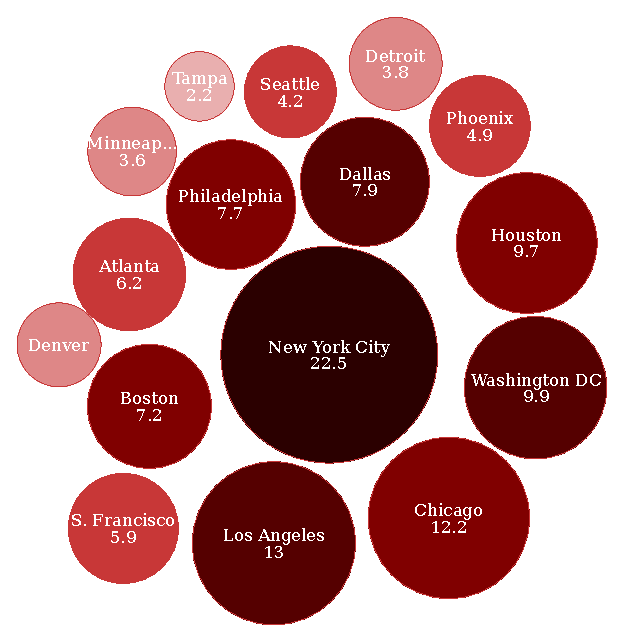
\includegraphics{img/time-cost.eps}
\caption[Tempo de espera acumulado (em anos)]{\label{fig:timecost}Tempo de espera acumulado (em anos) por elevadores
durante 12 meses em 16 cidades norte-americanas. Fonte:~\cite{IBM10}}
\end{figure}

Neste contexto global, a indústria de elevadores possui alguns desafios:
primeiro, lidar com a pressão para a redução de custos na construção civil,
construindo sistemas de grupos de elevadores mais baratos e eficientes, com
melhorias no desempenho de transporte; segundo, competir no mercado oferecendo
serviços novos, personalizados e com garantia de qualidade, visando revolucionar
a maneira com que elevadores interagem e servem
passageiros~\cite{KOEHLEROTTIGER02}. Já sob o ponto de vista dos passageiros,
estes esperam que suas chamadas sejam atendidas imediatamente e que sejam
levados ao seu destino o mais rápido possível. Portanto, melhorias no desempenho
destes sistemas traduzem-se em alto valor tanto para os fabricantes quanto para
os usuários de elevadores.

Existem diversas abordagens que os fabricantes de elevadores podem usar para
tornar o sistema mais eficiente. Por exemplo, projetar o sistema com um número
maior de elevadores ou optar por elevadores com maior capacidade de carga.
Entretanto, este tipo de alteração não é sempre realizável em função de
limitações na estrutura do prédio ou inviabilidade financeira. Uma solução de
mais fácil aplicação é otimizar o sistema de controle dos elevadores.

A função deste sistema é resolver um problema de otimização: atribuir elevadores
para atender chamadas feitas pelos passageiros minimizando alguma métrica - mais
adiante serão apresentadas as métricas de desempenho utilizadas. Entretanto,
este problema encontra-se no conjunto de problemas NP-difícil (ou NP-hard, ou
NP-completo)~\cite{SeKo99}. Portanto, uma solução ótima, computável em tempo
polinomial, ainda não é conhecida para este problema.

Desde meados dos anos 1980, a indústria de elevadores vem estudando e
implementando estratégias para encontrar soluções sub-ótimas para o problema de
otimização. Diversas técnicas de Inteligência Artificial foram adotadas, como
redes neurais, algoritmos genéticos, lógicas \textit{fuzzy} e, mais
recentemente, sistemas multi-agentes, planejamento e aprendizado de
máquina~\cite{KOEHLEROTTIGER02}. Porém, melhorias significativas apenas são
encontradas nos modelos de ponta, que adotam novos paradigmas de utilização e
interface com usuários, e acabam ausentes dos modelos mais simples e
legados, i.e.,~que já estão instalados nos prédios.

Ao analisar a tecnologia atual, percebe-se que houve pouca evolução nos
elevadores desde sua concepção~-~sobretudo nos sistemas mais simples e mais
baratos. De fato, o mecanismo que os faz mover evoluiu drasticamente, fato
evidenciado ao comparar máquinas de tração manual com máquinas elétricas
modernas. No entanto, essas evoluções são de difícil percepção aos usuários de
elevadores. O sistema de controle dos elevadores ainda é simples, utilizando-se
muito pouco de técnicas de Inteligência Artificial para alterar seu
comportamento em tempo de execução, apesar dos esforços da indústria ao longo
das últimas décadas.

Acredita-se que tais técnicas permitam trazer uma evolução grande para os
sistemas de controle de grupos de elevadores, assim como os motores elétricos
foram para a tração. Por isto, o objetivo desde trabalho é comparar, através de
simulações, diferentes estratégias de controle de elevadores utilizando
Inteligência Artificial em alguns cenários. Assim, espera-se ser possível
avaliar, dentre as opções possíveis, quais combinações resultam em um melhor
desempenho no transporte de passageiros para cada cenário.

\section{\label{section:motivation}Motivação Prática}

O uso de elevadores é presente na vida de grande parte dos habitantes de grandes
metrópoles. Uma parcela significativa do dia-a-dia desta população é passada em
grandes caixas metálicas, ou esperando pelas mesmas. A possibilidade de aplicar
conhecimentos em Inteligência Artificial para melhorar o desempenho deste meio
de transporte e, por conseqüência, contribuir com um aumento na qualidade de
vida de seus passageiros é um grande atrativo para o estudo deste assunto.

Além disso, a Inteligência Artifical é uma área de conhecimento de grande
interesse dos autores, junto dos problemas relacionados a simulações, às
ferramentas de programação e à engenharia de software. O problema de otimização
na alocação de elevadores apresenta um campo de pesquisa único para a aplicação
destas ferramentas em busca da prática da Inteligência Artificial.
